
\documentclass[11pt]{article}
\usepackage[paper=letterpaper, margin=.5in]{geometry}
\pdfpagewidth 8.5in
\pdfpageheight 11in
\setlength\parindent{0in}

%%% Packages
% First four - AMS (american mathematical society). General math goodness. I use the align* enviorment in particular
% multirow, multicol allow for certain kinds of tables
% enumerate lets you determine the style of the counter for the enumerate enviorment
% graphicx lets you include pictures
% listings lets you stick in blocks of code
% placeins defines "\FloatBarrier", which stops tables from moving around
\usepackage{amsmath, amscd, amssymb, amsthm, multirow, multicol, enumerate, graphicx, listings, placeins} 
\newcommand{\Z}{\mathbb{Z}}
\newcommand{\R}{\mathbb{R}}
\newcommand{\Q}{\mathbb{Q}}
\newcommand{\C}{\mathbb{C}}
\newcommand{\N}{\mathbb{N}}
\newcommand{\V}{\mathbb{V}}
\newcommand{\U}{\mathcal{U}}
\newcommand{\del}{\partial}
\newcommand{\real}{\textrm{Re }}
\newcommand{\imag}{\textrm{Im }}
\newcommand{\pd}[2]{\frac{\partial #1}{\partial #2}}
\newcommand{\deriv}[2]{\frac{d #1}{d #2}}
\newcommand{\sumk}{\sum_{k=1}^\infty}
\newcommand{\sumj}{\sum_{j=1}^\infty}
\newcommand{\sumn}{\sum_{n=0}^\infty}
\newcommand{\summ}[2]{\sum_{k=#1}^{#2}}
\newcommand{\sig}[1]{\sum_{#1 =1}^\infty}
\newcommand{\un}[1]{\bigcup_{#1 =1}^\infty}
\newcommand{\inter}[1]{\bigcap_{#1 =1}^\infty}
\newcommand{\ip}[2]{\langle #1, #2 \rangle}
\newcommand{\ipxu}{\langle x,u_j \rangle}
\newcommand{\uj}{\{u_j\}_{j=1}^\infty}
\newcommand{\B}{\mathcal{B}}

\newcommand{\E}{\mathrm{E}}
\newcommand{\var}{\mathrm{Var}}
\newcommand{\cov}{\mathrm{Cov}}
\newcommand{\ST}{mbox{ s.t. }}

\newcommand{\Example}{\noindent {\bf Example. \quad} }
\newcommand{\Proof}{\noindent {\bf Proof: \quad} }
\newcommand{\Remark}{\noindent {\bf Remark. \quad} }
\newcommand{\Remarks}{\noindent {\bf Remarks. \quad} }
\newcommand{\Case}{\noindent {\underline{Case} \quad} }

\newcommand{\st}{ \; \big | \:}

\newcommand{\deuc}{d_{\mathrm euc}}
\newcommand{\dtaxi}{d_{\mathrm taxi}}
\newcommand{\ddisc}{d_{\mathrm disc}}
\newtheorem{theorem}{Theorem}[section]
\newtheorem{lemma}[theorem]{Lemma}
\newtheorem{proposition}[theorem]{Proposition}
\newtheorem{corollary}[theorem]{Corollary}
\theoremstyle{definition}
\newtheorem{definition}[theorem]{Definition}
\newtheorem{example}[theorem]{Example}

\begin{document}

%%%%%%%%%%%%%%%%%%%%%%%%%%%%%%%%%%%%%%%%%%%%%%%%%%%%%%%%%%%%%%%%%%%%%%%%%%%%%%%%%%%%%%%%%%%%%%%%%%%%%%%%%%%%%%%%%%%%%%%%%%%%%%%%%%%%%

STAT 343 Homework 8 \hfill Aaron Maurer
\vspace{2mm}
\hrule
\vspace{2mm}

\begin{itemize}
    \item[1.]
        \begin{itemize}
            \item[(a)]
                As we have proved, if the matix $X$ isn't singular, then the least squares solution from OLS is unique and indeed the optimal fit. Thus, if a $\beta$ acheives the minimum least squares, it must be the OLS coefficient from the regression. Calculating the sum of squares for a coefficient $\hat\beta ^{(-i)}$ on $\tilde Y^{(-i)}$, we get 
                \begin{align*}
                    \|\tilde Y^{(-i)} - X\hat\beta^{(-i)}\|^2 &= (x_i\beta^{(-i)} - x_i\beta^{(-i)})^2 + \|Y^{(-i)} - X^{(-i)}\hat\beta ^{(-i)}\|^2 \\
                    \|\tilde Y^{(-i)} - X\hat\beta^{(-i)}\|^2 &= \|Y^{(-i)} - X^{(-i)}\hat\beta^{(-i)}\|^2
                \end{align*}
                Since the sum on the right is the minimum possible over all $\beta$ (since the coefficient was fit by OLS on $Y^{(-i)}$), $\hat\beta ^{(-i)}$ minimizes the sum of squares for $\tilde Y^{(-i)}$. By our earlier reasoning, it thus must be the coefficient that would result from OLS run predicting $\tilde Y^{(-i)}$ in terms of $X$. 
            \item[(b)]
                The prediction of a linear model with coefficient $\hat\beta ^{(-i)}$ at point $x_i^T$ is $x_i^T\hat\beta ^{(-i)}$, so since that is the coefficient for regressing $\tilde Y^{(-i)}$ on $X$, $x_i^T\hat\beta ^{(-i)}$ will be the fit.

        \end{itemize}
    \item[2.]
        \begin{itemize}
            \item[(a)]
                \begin{align*}
                    \hat y_i-\hat f^{(-i)}(x_i) &= y_i- S(x_i)^{(-i)}Y^{(-i)} \\
                    \hat y_i-\hat f^{(-i)}(x_i) &= y_i- \frac{1}{\sum_{j\neq i} S_{ij}} \sum_{j\neq i} y_j S_{ij} \\
                    \hat y_i-\hat f^{(-i)}(x_i) &= y_i- \frac{\hat f(x_i)-y_iS_{ii}(X)}{1-S_{ii}} \\
                    \hat y_i-\hat f^{(-i)}(x_i) &= \frac{y_i - y_i S_{ii} - \hat f (x) + y_iS_{ii}}{1- S_{ii}} \\
                    \hat y_i-\hat f^{(-i)}(x_i) &= \frac{y_i -\hat f (x) }{1- S_{ii}} \\
                \end{align*}
            \item[(b)]
                Rather than refitting the regression $n$ times to estimate the leave one out cross validation estimate of error, this allows the regression to merely be fit once, saving a lot of costly $QR$ factorization or matrix inversion.
            \item[(c)]
                Since $1\geq1-S_{ii}\geq0$, we have 
                \begin{align*}
                    \vert y_i - \hat f(x_i) \vert &\leq \frac{\vert y_i - \hat f(x_i) \vert }{1-S_{ii}} \\
                    \vert y_i - \hat f(x_i) \vert &\leq \left\vert\frac{y_i - \hat f(x_i) }{1-S_{ii}} \right\vert  \\
                    \vert y_i - \hat f(x_i) \vert &\leq \left\vert y_i - \hat f^{(-i)}(x_i)\right\vert  
                \end{align*}

        \end{itemize}
    \item[3.]
        \begin{itemize}
            \item[(a)]
                Applying backwards elimination with a critical value of $.2$, we only remove the variable status. After that, all predictors have a p-value of less than $.2$, so we stop. \\
                \smallskip
                
                p-value at the point of exclusion: \\
                \FloatBarrier
                % latex table generated in R 3.1.1 by xtable 1.7-4 package
% Wed Dec  3 08:54:10 2014
\begin{table}[ht]
\centering
\begin{tabular}{rrr}
  \hline
 & Order & p-value \\ 
  \hline
status & 1.000 & 0.853 \\ 
   \hline
\end{tabular}
\end{table}
 
                \FloatBarrier

                Resulting model: \\
                \FloatBarrier
                % latex table generated in R 3.1.1 by xtable 1.7-4 package
% Wed Dec  3 08:54:10 2014
\begin{table}[ht]
\centering
\begin{tabular}{rrrrr}
  \hline
 & Estimate & Std. Error & t value & Pr($>$$|$t$|$) \\ 
  \hline
(Intercept) & 24.139 & 14.769 & 1.634 & 0.109 \\ 
  sex & -22.960 & 6.771 & -3.391 & 0.002 \\ 
  income & 4.898 & 0.955 & 5.128 & 0.000 \\ 
  verbal & -2.747 & 1.825 & -1.505 & 0.140 \\ 
   \hline
\end{tabular}
\end{table}
 
                \FloatBarrier

            \item[(b)]
                For each of the following three methods, I used an exhaustive subset search, which determined which set of a particular number of variables resulted in the smallest RSS. The result, which is a boolean indicating whether the predictor should be included at each number of predictors is below. Since this will uniformly be the best model of $n$ predictors, the remaining decision is which $n$ to use. It should be noted that the model in a is indeed the optimal model of $3$ predictors. \\
                \FloatBarrier
                % latex table generated in R 3.1.1 by xtable 1.7-4 package
% Wed Dec  3 08:54:11 2014
\begin{table}[ht]
\centering
\begin{tabular}{rlllll}
  \hline
 & (Intercept) & sex & status & income & verbal \\ 
  \hline
1 & TRUE & FALSE & FALSE & TRUE & FALSE \\ 
  2 & TRUE & TRUE & FALSE & TRUE & FALSE \\ 
  3 & TRUE & TRUE & FALSE & TRUE & TRUE \\ 
  4 & TRUE & TRUE & TRUE & TRUE & TRUE \\ 
   \hline
\end{tabular}
\end{table}
 
                \FloatBarrier
                The model with the lowest AIC also had $3$ predictors, and is thus the same as in a. The different AICs for the best model with $n$ predictors  below. \\
                \FloatBarrier
                % latex table generated in R 3.1.1 by xtable 1.7-4 package
% Wed Dec  3 08:54:11 2014
\begin{table}[ht]
\centering
\begin{tabular}{rrrrr}
  \hline
 & 1 & 2 & 3 & 4 \\ 
  \hline
Predictors & 1.000 & 2.000 & 3.000 & 4.000 \\ 
  AIC & 304.336 & 296.627 & 296.214 & 298.176 \\ 
   \hline
\end{tabular}
\end{table}
 
                \FloatBarrier

            \item[(c)]
                The model with the highest adjusted $R^2$ is this same model with $3$ predictors. Optimal adjusted $R^2$ for different number of predictors are below. \\
                \FloatBarrier
                % latex table generated in R 3.1.1 by xtable 1.7-4 package
% Wed Dec  3 08:54:11 2014
\begin{table}[ht]
\centering
\begin{tabular}{rrrrr}
  \hline
 & 1 & 2 & 3 & 4 \\ 
  \hline
Predictors & 1.000 & 2.000 & 3.000 & 4.000 \\ 
  Adjusted R Squared & 0.373 & 0.479 & 0.493 & 0.482 \\ 
   \hline
\end{tabular}
\end{table}
 
                \FloatBarrier


            \item[(d)]
                Going by Mallow's $C_p$, we once again get the same model. The smallest model that had a $C_p$ smaller than the number of parameters (one more than the number of predictors due to the intercept) was the model with 3 predictors (4 parameters): \\
                \FloatBarrier
                % latex table generated in R 3.1.1 by xtable 1.7-4 package
% Wed Dec  3 08:54:11 2014
\begin{table}[ht]
\centering
\begin{tabular}{rrrrr}
  \hline
 & 1 & 2 & 3 & 4 \\ 
  \hline
Parameters & 2.000 & 3.000 & 4.000 & 5.000 \\ 
  Mallow's Cp & 11.401 & 3.248 & 3.035 & 5.000 \\ 
   \hline
\end{tabular}
\end{table}
 
                \FloatBarrier
        \end{itemize}
    \item[4.]
        The order of these operations doesn't make much difference. Point 21 is influential both before and after model selection, and the prefered model includes Air.Flow and Water.Temp, while excluding Acid.Conc, whether or not the outlier is included. \\
        \smallskip
        Our initial model is below. Acid.Conc looks ripe to be removed with a high $p-value$
        \FloatBarrier
        % latex table generated in R 3.1.1 by xtable 1.7-4 package
% Wed Dec  3 10:04:52 2014
\begin{table}[ht]
\centering
\begin{tabular}{rrrrr}
  \hline
 & Estimate & Std. Error & t value & Pr($>$$|$t$|$) \\ 
  \hline
(Intercept) & -39.920 & 11.896 & -3.356 & 0.004 \\ 
  Air.Flow & 0.716 & 0.135 & 5.307 & 0.000 \\ 
  Water.Temp & 1.295 & 0.368 & 3.520 & 0.003 \\ 
  Acid.Conc. & -0.152 & 0.156 & -0.973 & 0.344 \\ 
   \hline
\end{tabular}
\end{table}
 
        \FloatBarrier
        Indeed, when we test all subsets of the data, it is excluded from every model that has fewer than three predictors:
        \FloatBarrier
        % latex table generated in R 3.1.1 by xtable 1.7-4 package
% Wed Dec  3 10:04:52 2014
\begin{table}[ht]
\centering
\begin{tabular}{rllll}
  \hline
 & (Intercept) & Air.Flow & Water.Temp & Acid.Conc. \\ 
  \hline
1 & TRUE & TRUE & FALSE & FALSE \\ 
  2 & TRUE & TRUE & TRUE & FALSE \\ 
  3 & TRUE & TRUE & TRUE & TRUE \\ 
   \hline
\end{tabular}
\end{table}
 
        \FloatBarrier
        The optimal subset, when going by adjusted $R^2$ is the model with just two predictors ($R^2$ for each optimal subset of a particular size below):
        \FloatBarrier
        % latex table generated in R 3.1.1 by xtable 1.7-4 package
% Wed Dec  3 10:04:52 2014
\begin{table}[ht]
\centering
\begin{tabular}{rr}
  \hline
 & x \\ 
  \hline
1 & 0.838 \\ 
  2 & 0.899 \\ 
  3 & 0.898 \\ 
   \hline
\end{tabular}
\end{table}
 
        \FloatBarrier
        Choosing this as our model, we get the following model:
        \FloatBarrier
        % latex table generated in R 3.1.1 by xtable 1.7-4 package
% Wed Dec  3 10:04:52 2014
\begin{table}[ht]
\centering
\begin{tabular}{rrrrr}
  \hline
 & Estimate & Std. Error & t value & Pr($>$$|$t$|$) \\ 
  \hline
(Intercept) & -50.359 & 5.138 & -9.801 & 0.000 \\ 
  Air.Flow & 0.671 & 0.127 & 5.298 & 0.000 \\ 
  Water.Temp & 1.295 & 0.367 & 3.525 & 0.002 \\ 
   \hline
\end{tabular}
\end{table}
 
        \FloatBarrier
        Checking the distribution of studentized residuals for outliers, we see one potential culprit (the largest residual, in the top right, which heavily deviates from T-distribution).
        \begin{center}
            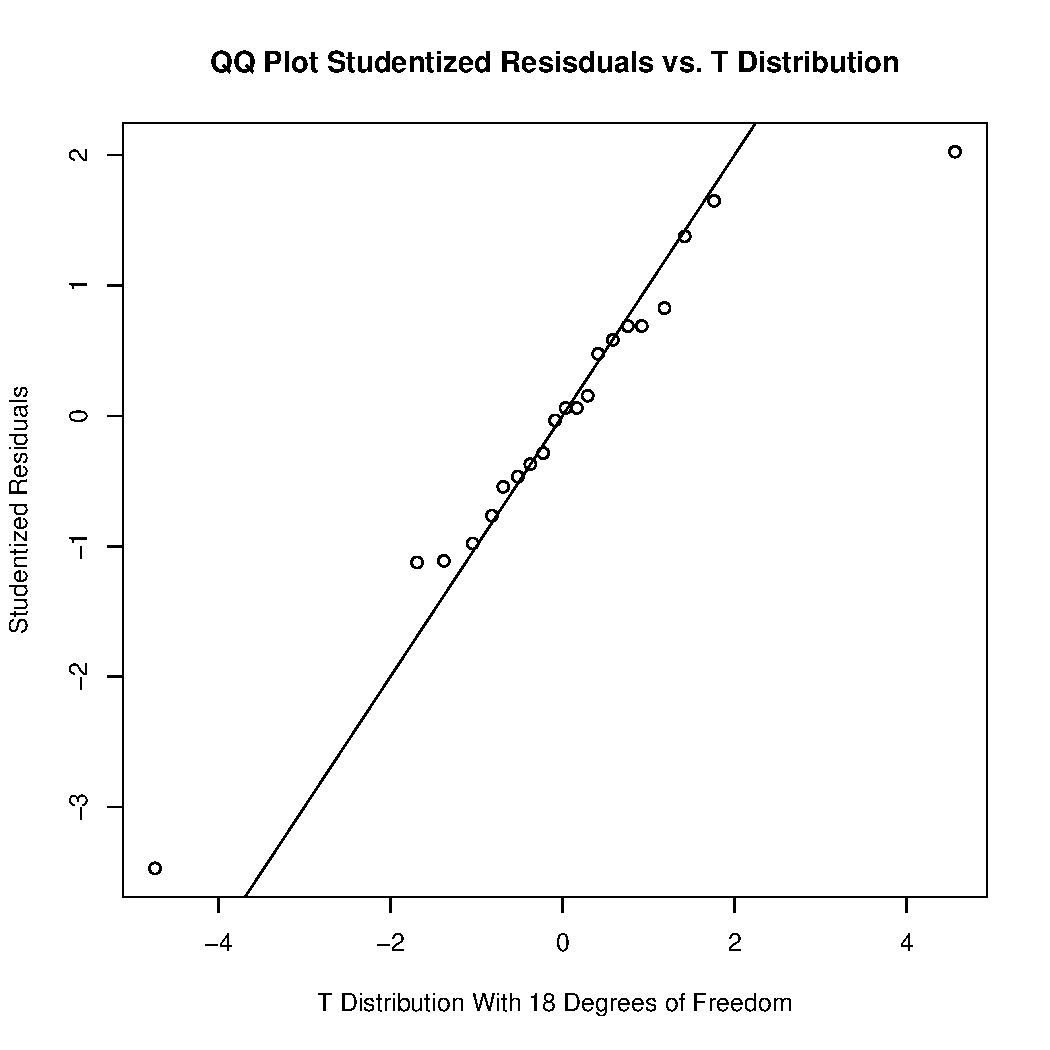
\includegraphics[width=9cm]{hw8/hw8_4_small_rstudent} 
        \end{center}
        It is the 21st data point. With a studentized residual value of $-3.47$, it is just inside conservative Bonferroni critical value, for $\alpha=.5$, of $-3.53$. Thus, we don't quite reject it as an outlier. However, looking at the plot of Cook's distances, it is clear that the same point is highly influential.
        \begin{center}
            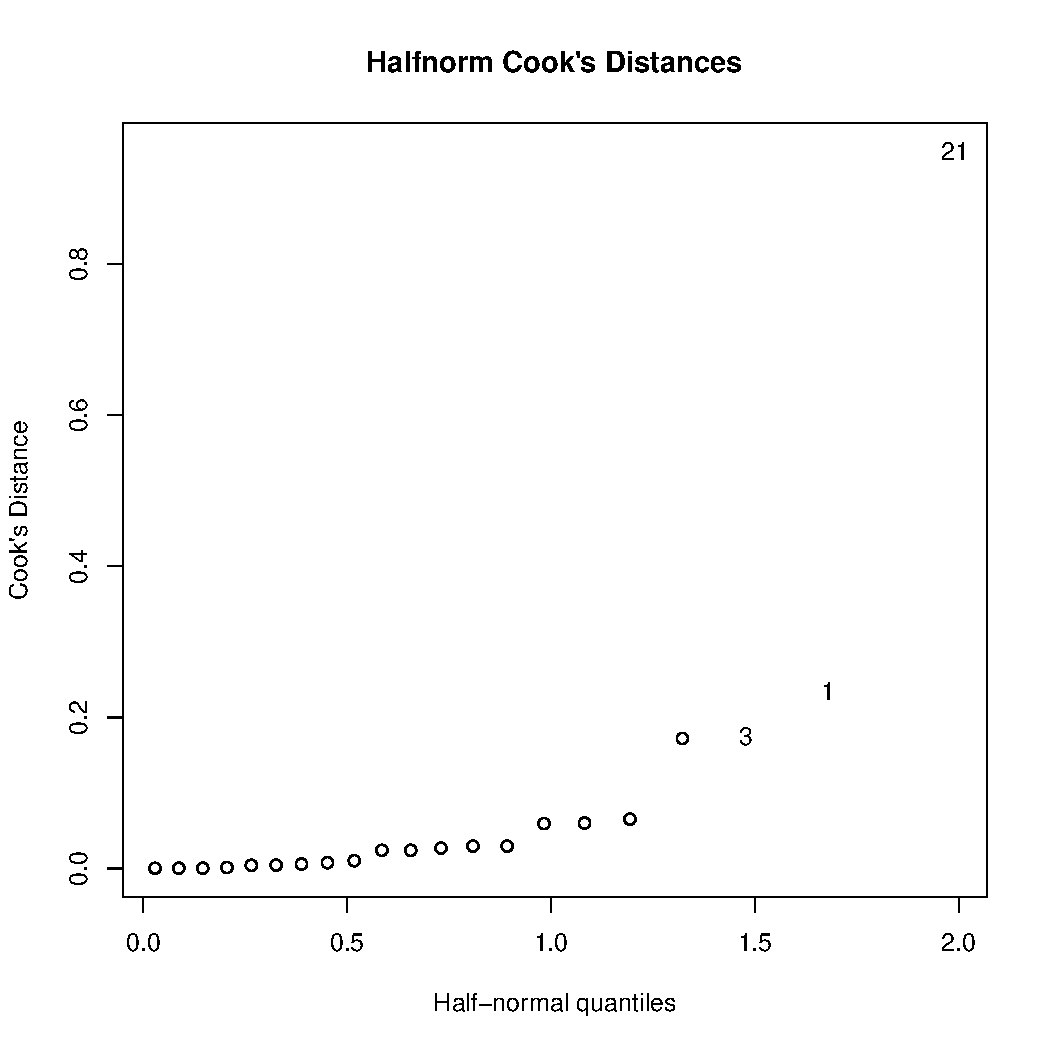
\includegraphics[width=9cm]{hw8/hw8_4_small_cook}
        \end{center}
        Now, going back to the full model which included Acid.Conc, we look again for outliers and influential points. Shockingly, the same point is once again the only real canidate. The distribution of studentized residuals on this
        \begin{center}
            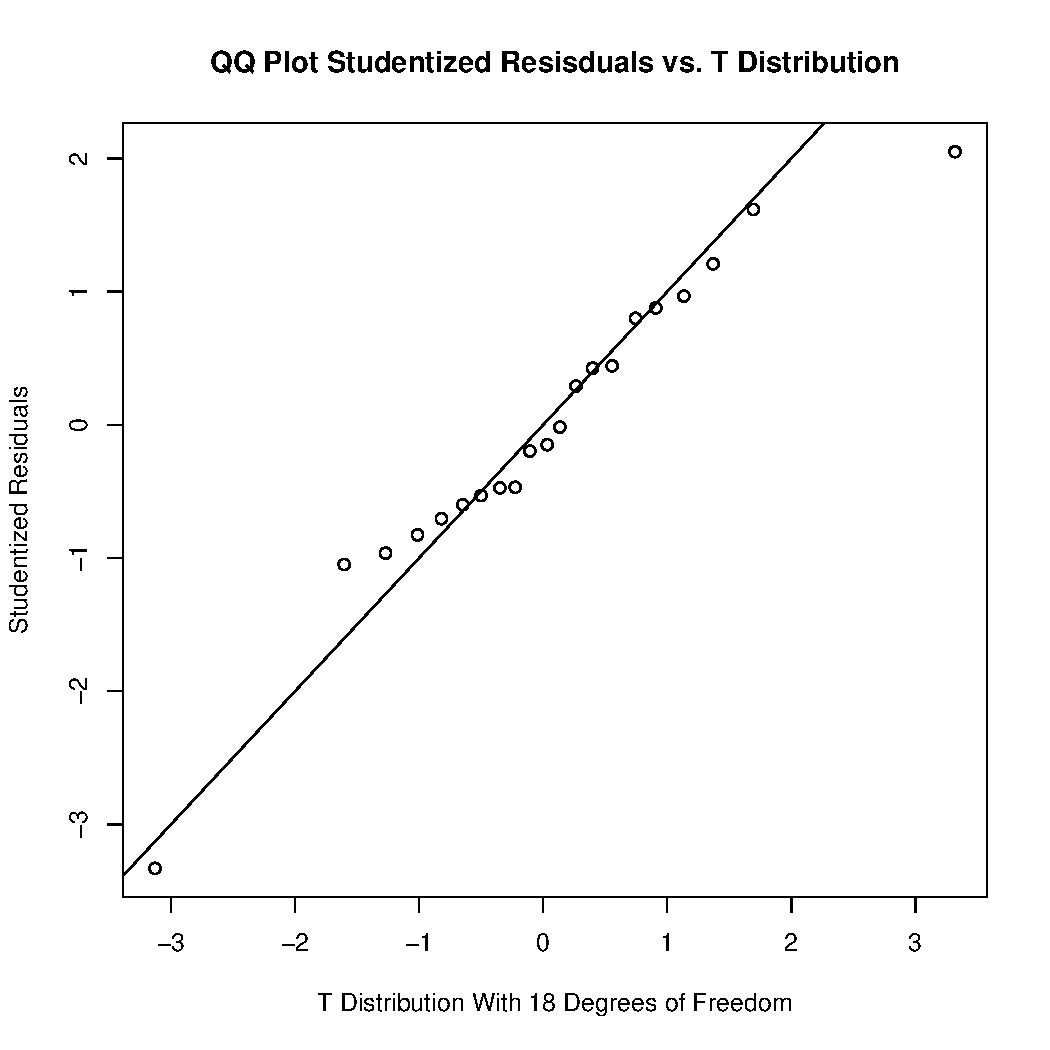
\includegraphics[width=9cm]{hw8/hw8_4_rstudent} 
        \end{center}
        Testing it as an outlier as before, it has a studentized residual of $-3.33$ in this model, while the critical value is $-3.54$, so we don't reject it. However, its still influential, so we kick it out for that:
        \begin{center}
            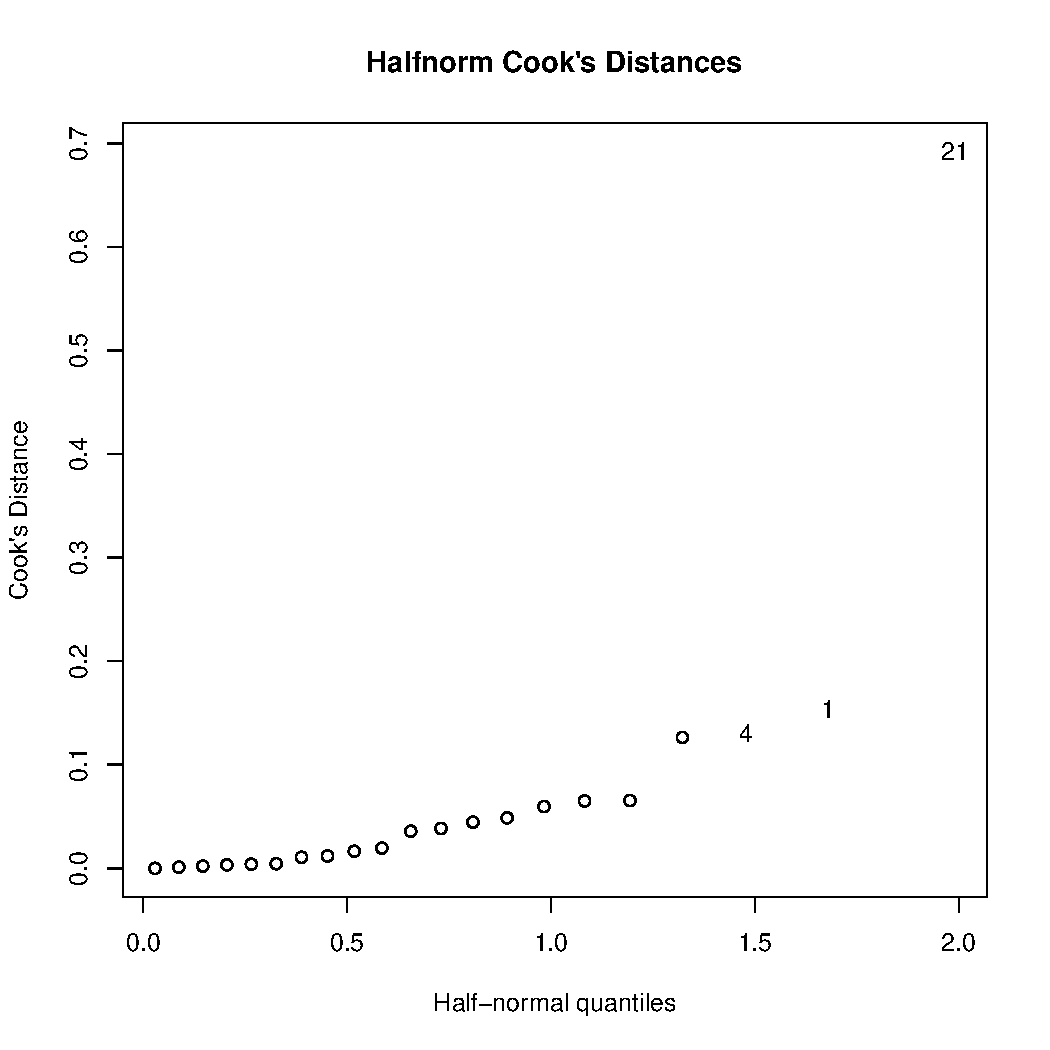
\includegraphics[width=9cm]{hw8/hw8_4_cook}
        \end{center}
        Preforming variable selection on the data set with this point excluded, we still find the optimal model has the two variables besides Acid.Conc. Optimal subsets of each size:
        \FloatBarrier
        % latex table generated in R 3.1.1 by xtable 1.7-4 package
% Wed Dec  3 10:04:52 2014
\begin{table}[ht]
\centering
\begin{tabular}{rllll}
  \hline
 & (Intercept) & Air.Flow & Water.Temp & Acid.Conc. \\ 
  \hline
1 & TRUE & TRUE & FALSE & FALSE \\ 
  2 & TRUE & TRUE & TRUE & FALSE \\ 
  3 & TRUE & TRUE & TRUE & TRUE \\ 
   \hline
\end{tabular}
\end{table}
 
        \FloatBarrier
        Adjusted $R^2$ for these subsets, showing we still prefer the model with two predictors:
        \FloatBarrier
        % latex table generated in R 3.1.1 by xtable 1.7-4 package
% Wed Dec  3 10:04:52 2014
\begin{table}[ht]
\centering
\begin{tabular}{rr}
  \hline
 & x \\ 
  \hline
1 & 0.923 \\ 
  2 & 0.940 \\ 
  3 & 0.939 \\ 
   \hline
\end{tabular}
\end{table}
 
        \FloatBarrier
    \item[5.]
        \begin{itemize}
            \item[(a)]
                I have plotted the singular values below, gotten by taking the square roots of the absolute values of the eigenvalues of $XX^T$ (once $X$ had been centered). They quickly fall off to very small values, reflecting that most of the variation in the data set is explained by just a few underlying components.
                \begin{center}
                    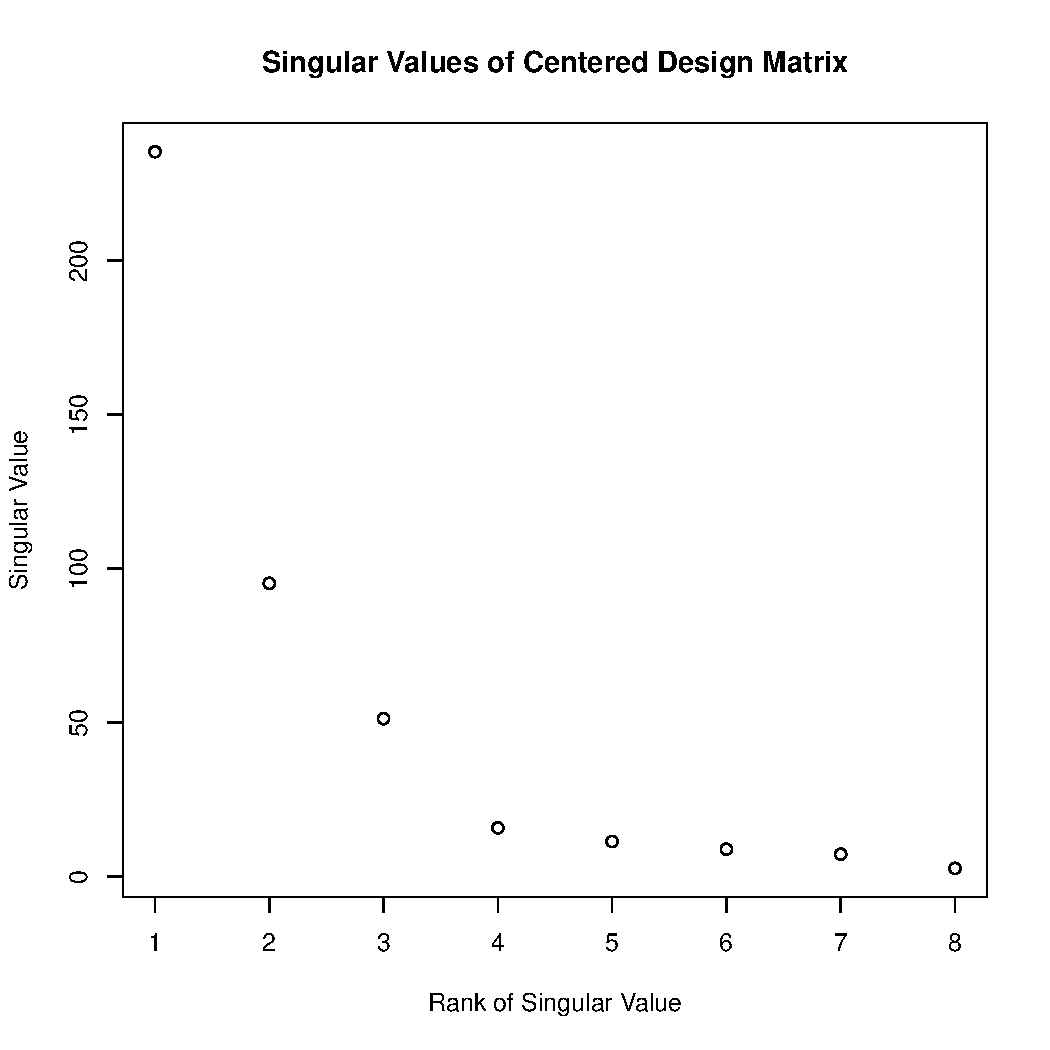
\includegraphics[width=9cm]{hw8/5_a}
                \end{center}
            \item[(b)]
                The components of the two largest singular vectors are plotted below. As would be expected, the components of the second vector are generally far smaller than those of the first. It appears that approximately half the time the second component has the same sign as the first, and half the time the opposite sign, as might be expected since they are orthogonal. The vaguely resemble piecies of orthogonal waves.  
                \begin{center}
                    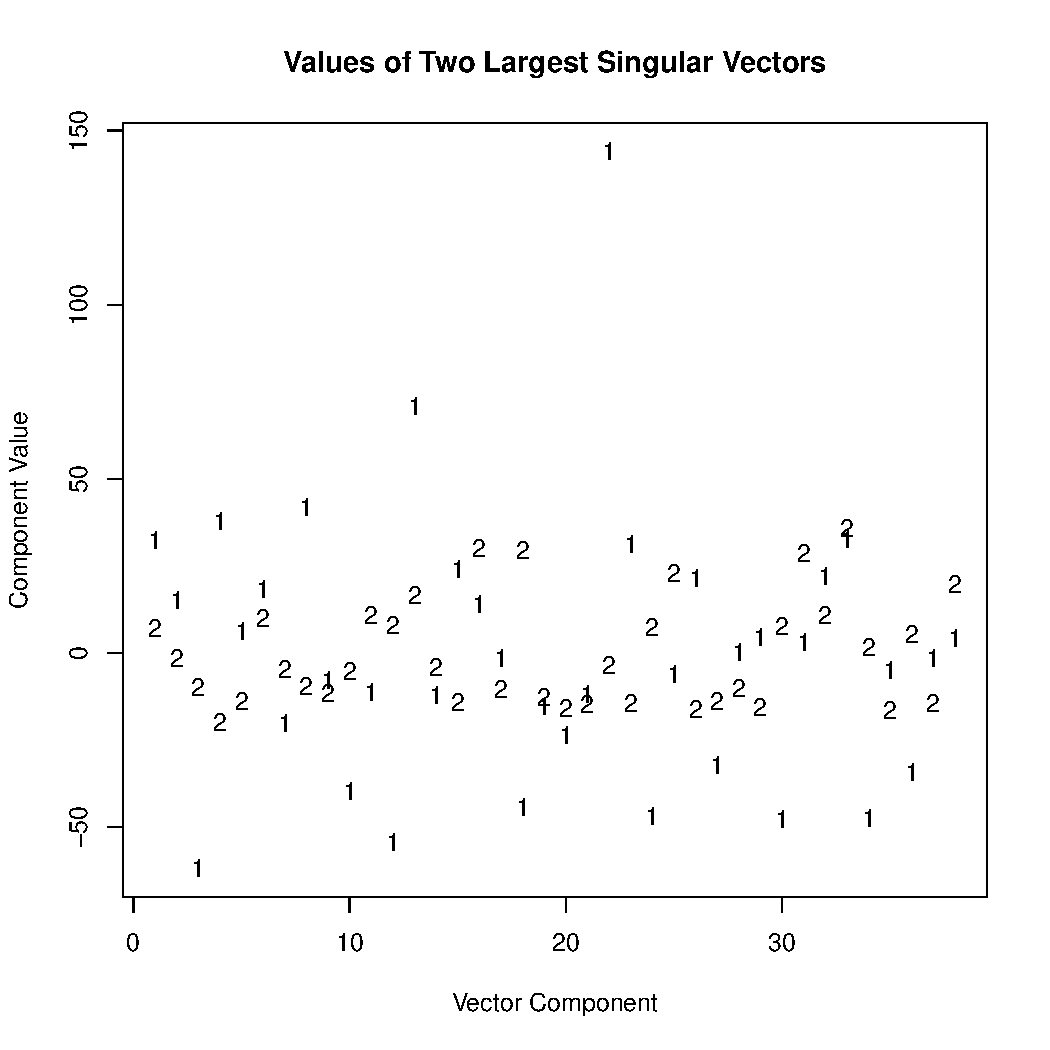
\includegraphics[width=9cm]{hw8/5_b}
                \end{center}

            \item[(c)] 
            We see that the regression on the two largest princple components doesn't actually predict the data as well as the two best predictors from the original data set (for the same number of variables, the latter has higher $R^2$). While this latter model predicts almost as well as the model including all variables, the largest principle components are signficantly less predictive, though still reasonably predictive. The reason for this is that the principle components are a decomposition of variation within the predictors; however, the largest source of variation in these predictors isn't necessarily predictive of the outcome. For instance, if there is a lot of variation among a few variables that aren't predictive of the outcome, they may correspond to large principle components, but these principle components will likely be also unpredictive. On the other hand, since the principle components as a whole define a space equivalent to the orginal space defined by all the predictors, a model including all of them will be equally predictive to including all variables.  \\
            \smallskip
            The regression on the two largest principle components ($R^2=.5469$):
            \FloatBarrier
            % latex table generated in R 3.1.1 by xtable 1.7-4 package
% Wed Dec  3 11:31:27 2014
\begin{table}[ht]
\centering
\begin{tabular}{rrrrr}
  \hline
 & Estimate & Std. Error & t value & Pr($>$$|$t$|$) \\ 
  \hline
(Intercept) & -164.885 & 6.697 & -24.622 & 0.000 \\ 
  PCPC1 & -1.049 & 0.175 & -5.984 & 0.000 \\ 
  PCPC2 & 1.099 & 0.433 & 2.537 & 0.016 \\ 
   \hline
\end{tabular}
\end{table}
 
            \FloatBarrier
            The regression on all variables ($R^2=.6866$):
            \FloatBarrier
            % latex table generated in R 3.1.1 by xtable 1.7-4 package
% Wed Dec  3 11:31:27 2014
\begin{table}[ht]
\centering
\begin{tabular}{rrrrr}
  \hline
 & Estimate & Std. Error & t value & Pr($>$$|$t$|$) \\ 
  \hline
(Intercept) & 436.432 & 166.572 & 2.620 & 0.014 \\ 
  Age & 0.776 & 0.570 & 1.360 & 0.184 \\ 
  Weight & 0.026 & 0.331 & 0.080 & 0.937 \\ 
  HtShoes & -2.692 & 9.753 & -0.276 & 0.784 \\ 
  Ht & 0.601 & 10.130 & 0.059 & 0.953 \\ 
  Seated & 0.534 & 3.762 & 0.142 & 0.888 \\ 
  Arm & -1.328 & 3.900 & -0.341 & 0.736 \\ 
  Thigh & -1.143 & 2.660 & -0.430 & 0.671 \\ 
  Leg & -6.439 & 4.714 & -1.366 & 0.182 \\ 
   \hline
\end{tabular}
\end{table}
 
            \FloatBarrier
            The regression on age and height ($R^2=.6562$):
            \FloatBarrier
            % latex table generated in R 3.1.1 by xtable 1.7-4 package
% Wed Dec  3 11:31:27 2014
\begin{table}[ht]
\centering
\begin{tabular}{rrrrr}
  \hline
 & Estimate & Std. Error & t value & Pr($>$$|$t$|$) \\ 
  \hline
(Intercept) & 526.959 & 92.248 & 5.712 & 0.000 \\ 
  Age & 0.521 & 0.386 & 1.349 & 0.186 \\ 
  Ht & -4.200 & 0.531 & -7.906 & 0.000 \\ 
   \hline
\end{tabular}
\end{table}
 
            \FloatBarrier
        \end{itemize}
 
 
    

\end{itemize}

\end{document}
